\begin{figure}
\centering
\begin{tikzpicture}[declare function={f(\x,\y)=(\x)^2+(\y)^2;fx(\r,\t)=\r*cos(\t);fy(\r,\t)=\r*sin(\t);fz(\r,\t)=(\r)^2;ft(\y)=5+4*(\y-2);}]
\pgfmathsetmacro{\k}{2.4}
\begin{axis}[small,clip=false,axis lines=center,colormap={}{gray(0cm)=(0.6);gray(1cm)=(0.8);},view/h=110,xtick={\empty},ytick={\empty},ztick={\empty},xlabel={$x$},ylabel={$y$},zlabel={$z$},xlabel style={anchor=west},zlabel style={anchor={south}},enlargelimits=true,hide z axis]
\addplot3[z buffer=sort,surf,domain=0:2.6,domain y=-45:360]({fx(x,y)},{fy(x,y)},{fz(x,y)});
\addplot3[thick,domain y=-\k:\k](1,\y,{1+(\y)^2});
\addplot3[]coordinates {(1,\k,0)(1,\k,0)(1,\k,7)(1,-\k,7)(1,-\k,0)}node[pos=0.75,pin={[align=center]190:{\RL{مستوی}\\ $x=1$}}]{};
\addplot3[domain y=0.75:2](1,y,{ft(y)})node[pos=0,pin={-45:{\RL{مماسی خط}}}]{};
\addplot3[]coordinates{(1,2,5)}node[circ]{}node[right]{$(1,2,5)$};
\end{axis}
\end{tikzpicture}
\caption{مستوی \عددی{x=1} اور سطح \عددی{z=x^2+y^2} کے تقاطع منحنی کا نقطہ \عددی{(1,2,5)} پر  مماس۔}
\end{figure}

\begin{figure}
\centering
\begin{subfigure}{0.45\textwidth}
\centering
\begin{tikzpicture}[font=\small]
\pgfmathsetmacro{\a}{2.5}
\pgfmathsetmacro{\b}{1.25}
\pgfmathsetmacro{\t}{0.1}
\pgfmathsetmacro{\ang}{45}
\draw[fill=llgray](0,0)coordinate(aa)--++(\a,0)coordinate(bb)--++(\ang:\b)coordinate(cc)--++(-\a,0)coordinate(dd)--(0,0);
\draw(0,0)--++(0,-\t)coordinate(aaa)--++(\a,0)coordinate(bbb)--++(\ang:\b)coordinate(ccc)--(cc);
\draw[fill=llgray](aa)--(aaa)--(bbb)--(ccc)--(cc)--(bb)--(aa);
\draw(bb)--(bbb);
\draw(\a/2,-0.8) circle (0.3cm and 0.1cm);
\draw(\a/2-0.3,-0.8)--++(0,-0.5);
\draw(\a/2+0.3,-0.8)--++(0,-0.5);
\draw[fill=white](\a/2,-0.3)to [out=-135,in=110]++(0,-0.5) to [out=80,in=-45]++(0,0.5);
\draw(3/4*\a,\b/2)node[circ]{}node[pin=60:{$\frac{\partial^{\,2}f}{\partial x^2}+\frac{\partial^{\,2}f}{\partial y^2}=0$}]{};
\end{tikzpicture}
\caption{}
\end{subfigure}\hfill
\begin{subfigure}{0.45\textwidth}
\centering
\begin{tikzpicture}[font=\small]
\pgfmathsetmacro{\a}{2.5}
\pgfmathsetmacro{\b}{1.25}
\pgfmathsetmacro{\c}{0.6}
\pgfmathsetmacro{\t}{0.1}
\pgfmathsetmacro{\ang}{45}
\draw(0,0)coordinate(aa)--++(\a,0)coordinate(bb)--++(\ang:\b)coordinate(cc)--++(-\a,0)coordinate(dd)--++(\ang:-\b);
\draw(0,\c)coordinate(taa)--++(\a,0)coordinate(tbb)--++(\ang:\b)coordinate(tcc)--++(-\a,0)coordinate(tdd)--++(\ang:-\b);
\draw[fill=llgray,opacity=0.5](0,\c/2)coordinate(maa)--++(\a,0)coordinate(mbb)--++(\ang:\b)coordinate(mcc)--++(-\a,0)coordinate(mdd)--++(\ang:-\b);
\draw[dashed](0,\c/2-\t)--++(\ang:\b)--++(\a,0);
\draw[fill=llgray,opacity=0.5](0,\c/2-\t)--++(\a,0)--++(\ang:\b)--++(0,\t)--++(\ang:-\b)--++(-\a,0)--++(0,-\t);
\draw(aa)--(taa)  (bb)--(tbb)  (cc)--(tcc)  (dd)--(tdd);
\draw(1/2*\a,\b/2+\t)node[circ]{}node[pin={[pin distance=1cm]70:{$\frac{\partial^{\,2}f}{\partial x^2}+\frac{\partial^{\,2}f}{\partial y^2}+\frac{\partial^{\,2}f}{\partial z^2}=0$}}]{};
\end{tikzpicture}
\caption{مستوی کی سرحدی حرارت قابو کی گئی ہے۔}
\end{subfigure}
\caption{مستوی اور ٹھوس اجسام میں برقرار حال حرارت، مساوات لاپلاس کو مطمئن کرتی ہے۔}
\end{figure}

\begin{figure}
\centering
\begin{tikzpicture}[font=\small]
\pgfmathsetmacro{\a}{5.25}
\pgfmathsetmacro{\b}{3}
\draw[fill=llgray](0,0)--++(\a,0)--++(0,\b)--++(-\a,0)--+(0,-\b);
\draw(1.25,0.5)node[circ]{}node[left]{$(x_0,y_0)$}node[pin={[align=center,pin distance=0.25cm]80:{\RL{نقطہ جہاں}\\   \RL{\عددی{f} قابل تفرق ہے}}}]{}--++(2,0)node[pos=0.5,below]{$\Delta x=x-x_0$}--++(0,2)node[pos=0.5,right]{$\Delta y=y-y_0$}node[circ]{}node[right]{$(x,y)$}node[pin={[align=center,left]-170:{\RL{\عددی{(x_0,y_0)} کے}\\   \RL{قریب نقطہ}}}]{};
\end{tikzpicture}
\caption{
اگر \عددی{(x_0,y_0)} پر \عددی{f} قابل تفرق ہو تب قریبی نقطہ \عددی{(x,y)} پر \عددی{f} کی قیمت تقریباً\\
\عددی{f(x_0,y_0)+f_x(x_0,y_0)\Delta x+f_y(x_0,y_0)\Delta y} ہو گی۔
}
\end{figure}


\begin{figure}
\centering
\begin{tikzpicture}
\pgfmathsetmacro{\a}{2.75}
\pgfmathsetmacro{\b}{2}
\draw[-latex](0,0)--(3,0)node[right]{$x$};
\draw[-latex](0,0)--(0,2.5)node[left]{$y$};
\draw[fill=llgray,opacity=0.5](0.5,0.25)node[above right,black]{$R$}--++(\a,0)--++(0,\b)--++(-\a,0)--++(0,-\b);
\draw[-latex](0.5,0.25)++(\a/2,\b/2)--++(\a/2,0)node[pos=0.5,above]{$h$};
\draw[-latex](0.5,0.25)++(\a/2,\b/2)node[ocirc]{}node[below]{$(x_0,y_0)$}--++(0,\b/2)node[pos=0.5,left]{$k$};
\end{tikzpicture}
\caption{
مستوی \عددی{xy} میں مستطیل خطہ  \عددی{R}:
$\abs{x-x_0}\le h,\,\abs{y-y_0}\le k$
جہاں  میں ہم اپنی تخمین کے خلل کی کارآمد  حد بندی تلاش کر سکتے ہیں
}
\end{figure}

\begin{figure}
\centering
\begin{subfigure}{0.45\textwidth}
\centering
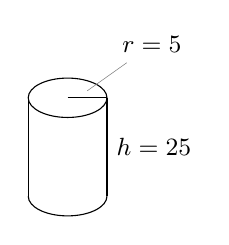
\begin{tikzpicture}[font=\small]
\pgfmathsetmacro{\ra}{0.5}
\pgfmathsetmacro{\rb}{\ra/2}
\pgfmathsetmacro{\h}{1.25}
\draw([shift={(180:\ra cm and \rb cm)}]0,0) arc (180:360:\ra cm and \rb cm);
\draw(0,\h) circle (\ra cm and \rb cm);
\draw(-\ra,0)--++(0,\h)  (\ra,0)--++(0,\h);
\draw(0,\h)--++(\ra,0)node[pos=0.25,pin=45:{$r=5$}]{};
\draw(\ra,\h/2)node[right]{$h=25$};
\end{tikzpicture}
\caption{}
\end{subfigure}\hfill
\begin{subfigure}{0.45\textwidth}
\centering
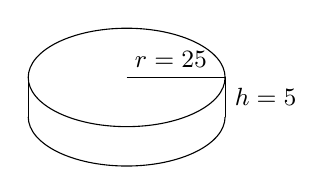
\begin{tikzpicture}[font=\small]
\pgfmathsetmacro{\ra}{1.25}
\pgfmathsetmacro{\rb}{\ra/2}
\pgfmathsetmacro{\h}{0.5}
\draw([shift={(180:\ra cm and \rb cm)}]0,0) arc (180:360:\ra cm and \rb cm);
\draw(0,\h) circle (\ra cm and \rb cm);
\draw(-\ra,0)--++(0,\h)  (\ra,0)--++(0,\h);
\draw(0,\h)--++(\ra,0)node[pos=0.45,above]{$r=25$};
\draw(\ra,\h/2)node[right]{$h=5$};
\end{tikzpicture}
\caption{}
\end{subfigure}
\caption{
بیلن-ا کا حجم \عددی{r} میں چھوٹی تبدیلی کو زیادہ حساس ہے جبکہ بیلن-ب کا حجم \عددی{h} میں چھوٹی تبدیلی کو زیادہ حساس ہے۔
}
\end{figure}

\begin{figure}
\centering
\begin{subfigure}{0.45\textwidth}
\centering
\begin{tikzpicture}[font=\small]
\pgfmathsetmacro{\r}{2.5}
\pgfmathsetmacro{\ang}{30}
\pgfmathsetmacro{\kx}{\r*cos(\ang)}
\pgfmathsetmacro{\ky}{\r*sin(\ang)}
\draw[-latex](0,0)--(3,0)node[right]{$x$};
\draw[-latex](0,0)--(0,2)node[left]{$y$};
\draw(0,0)--++(\ang:\r)node[pos=0.5,above left]{$r$}node[circ]{}node[above]{$N(3\mp0.01,4\mp0.01)$};
\draw[-stealth]([shift={(0:0.6)}]0,0) arc (0:\ang:0.6)node[pos=0.6,right]{$\theta$};
\draw(\kx,0)node[below]{$3$}--++(0,0.2);
\draw(0,\ky)node[left]{$4$}--++(0.2,0);
\end{tikzpicture}
\end{subfigure}\hfill
\begin{subfigure}{0.45\textwidth}
\centering
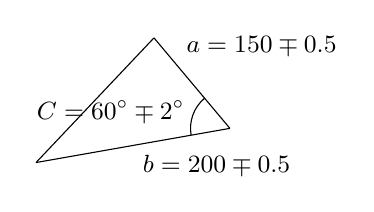
\begin{tikzpicture}[font=\small]
\pgfmathsetmacro{\a}{2.5}
\pgfmathsetmacro{\b}{1.5}
\pgfmathsetmacro{\angA}{10}
\pgfmathsetmacro{\angB}{50}
\draw(0,0)--++(180+\angA:\a)coordinate(a)node[pos=0.5,below right]{$b=200\mp 0.5$};
\draw(0,0)--++(180-\angB:\b)coordinate(b)node[pos=0.7,above right]{$a=150\mp 0.5$};
\draw(a)--(b);
\draw([shift={(180-\angB:0.5)}]0,0) arc (180-\angB:180+\angA:0.5)node[pos=0.4,left]{$C=60^{\circ}\mp 2^{\circ}$};
\end{tikzpicture}
\end{subfigure}
\end{figure}

\begin{figure}
\centering
\begin{tikzpicture}
\pgfmathsetmacro{\a}{1.75}
\pgfmathsetmacro{\b}{1.5}
\draw[-latex](0,0)--(3,0)node[right]{$x$};
\draw[-latex](0,0)--(0,2.5)node[left]{$y$};
\draw[fill=llgray,opacity=0.5](1,1)--++(\a,0)--++(0,\b)--++(-\a,0)--++(0,-\b);
\draw[-latex](1,1)++(\a/2,\b/2)--++(\a/2,0)node[pos=0.5,above]{$\dif r$};
\draw[-latex](1,1)++(\a/2,\b/2)node[ocirc]{}node[below]{$(5,12)$}--++(0,\b/2)node[pos=0.5,left]{$\dif h$};
\end{tikzpicture}
\end{figure}
